\documentclass[10pt,a4paper]{article}
\usepackage[margin=1.8cm]{geometry}
\usepackage{amsmath,amssymb,booktabs,graphicx,caption,xcolor,float,hyperref,tikz}
\usetikzlibrary{arrows.meta,calc}
\hypersetup{colorlinks=true,linkcolor=blue!50!black,urlcolor=blue!50!black}
\captionsetup{font=small,labelfont=bf}
\title{\vspace{-1.2cm}\textbf{Success against cost: an operational efficiency of control}\\[2pt]
\large DRAFT, for discussion --- Simulations 1 and 2, \texttt{task\_003}}
\author{LLM-free simulator; analysis of 13 October 2026}
\date{}
\begin{document}
\maketitle
\vspace{-1cm}

\paragraph{Summary.} Earlier information ratios (pair efficiency $\eta$, its variants, and the
action-based $\eta_U$) were either flat by construction or close to zero. Following the
operational proposal of the handoff document, we measure instead how much a controller changes the
probability that the swarm's \emph{collective decision} is its target (and the correct answer), and how
many facts it posts to do so. Three results stand out. (i)~\textbf{When no proof exists, success saturates
with very little control}: the cheapest controller reaches the full gain, and most configurations spend
two to four times more for nothing. (ii)~\textbf{Speed is worth paying for only early}: the efficiency
depends on when success is scored. (iii)~\textbf{Overturning a proof has increasing returns}: concentrated
control (random mixtures of strong control and none) beats every tested configuration.

\section{The simulators in brief}

24 agents, each given one true fact about \texttt{task\_003} (three allocations; A0 is correct), reason as
exact Bayesians and post facts on a shared board; a controller with a target (A0, truth; A2, false) posts
facts from its own pool. \textbf{Simulation 1}: days and nights; each agent reads $q$ posts a day, votes, and
posts a fact supporting its vote; each night the controller reads $q_c$ posts and, unless 75\% of them
already back its target (vote gate) or its target is proved (proof stop), posts $b$ facts; the board is
cleared nightly; memories fade at dawn (survival $\rho$). \textbf{Simulation 2}: no rounds; agents act at
random times (rate 1), the controller at rate $\lambda_c$ (one fact per message, at most 30, until
$t = 30$; gate on or off); memories fade continuously; readers see the 48 most recent posts. Agents
vote by probability matching; $q = 6$ throughout; 1{,}000 paired episodes per arm (silent, truth, false).

\section{Measures}

\begin{itemize}\itemsep1pt
\item \textbf{Collective decision} $Y_T$: plurality of the agents' last votes at time $T$; a tie between
  $k$ answers counts $1/k$. \textbf{Target attainment}: $Y_T$ = assigned target; \textbf{task
  correctness}: $Y_T$ = A0.
\item \textbf{Benefit} $\Delta_\pi = p_\pi - p_0$: change in the probability of success against the silent
  arm of the same episodes (scored with the same target).
\item \textbf{Cost} $C_\pi$: facts actually posted up to $T$, mean per run (not the allowed budget).
\item \textbf{Frontier} among the tested controller settings of one group (simulation, setup, $\rho$,
  target): $C^*(\delta) = \min\{C_\pi : \Delta_\pi \ge \delta\}$ and $\Delta^*(B) = \max\{\Delta_\pi : C_\pi \le B\}$;
  with \textbf{mixtures} (one configuration drawn per run) the frontier is the concave hull through $(0,0)$.
\item \textbf{Efficiencies}: $\eta_{\text{cost}} = C^*(\Delta_\pi)/C_\pi$ (share of the spending that was
  necessary), $\eta_{\text{perf}} = \Delta_\pi/\Delta^*(C_\pi)$, and \textbf{gain per fact} $\Delta_\pi/C_\pi$.
  Not defined where $\Delta_\pi \le 0$ or its 95\% interval includes 0.
\end{itemize}

\begin{center}
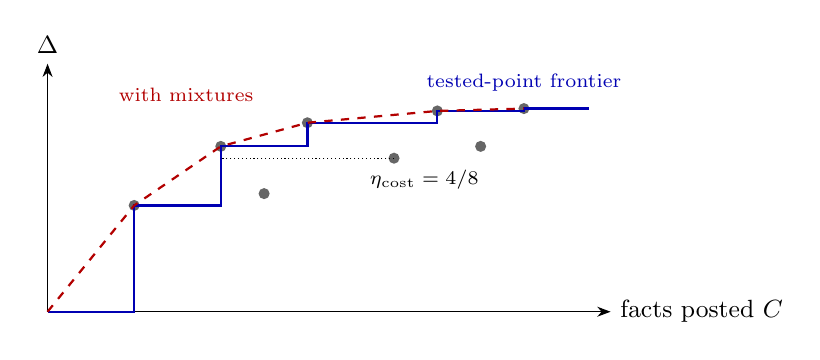
\begin{tikzpicture}[font=\small, x=0.55cm, y=3cm]
  \draw[-{Stealth}] (0,0) -- (13,0) node[right]{facts posted $C$};
  \draw[-{Stealth}] (0,0) -- (0,1.05) node[above]{$\Delta$};
  \foreach \c/\d in {2/0.45, 4/0.7, 6/0.8, 9/0.85, 11/0.86, 5/0.5, 8/0.65, 10/0.7}
     \fill[black!60] (\c,\d) circle (2pt);
  \draw[thick, blue!70!black] (0,0) -- (2,0) -- (2,0.45) -- (4,0.45) -- (4,0.7) -- (6,0.7) -- (6,0.8) -- (9,0.8) -- (9,0.85) -- (11,0.85) -- (11,0.86) -- (12.5,0.86);
  \draw[thick, dashed, red!70!black] (0,0) -- (2,0.45) -- (4,0.7) -- (6,0.8) -- (9,0.85) -- (11,0.86);
  \draw[densely dotted] (8,0.65) -- (4,0.65);
  \node[font=\scriptsize, align=left] at (8.7,0.56) {$\eta_{\text{cost}} = 4/8$};
  \node[font=\scriptsize, blue!70!black] at (11,0.97) {tested-point frontier};
  \node[font=\scriptsize, red!70!black] at (3.2,0.92) {with mixtures};
\end{tikzpicture}
\par\smallskip{\small\textbf{Diagram 1.} Each point is a configuration. The configuration at cost 8 reaches $\Delta = 0.65$, which a
configuration costing 4 already reaches: $\eta_{\text{cost}} = 0.5$.}
\end{center}

\section{Success against facts posted}

\begin{figure}[H]
\centering\includegraphics[width=\linewidth]{figures/frontier_target_T30.png}
\caption{Change in the probability that the controller's target wins, $t = 30$, against facts posted
(log scale), every configuration with its 95\% interval (blue: target A0; red: target A2; Simulation 2:
circles gate on, squares gate off). Solid: tested-point frontier; dashed: with mixtures.}
\label{fig:t30}
\end{figure}

\begin{figure}[H]
\centering\includegraphics[width=\linewidth]{figures/frontier_target_T5.png}
\caption{As Figure~\ref{fig:t30}, at $t = 5$.}
\label{fig:t5}
\end{figure}

\begin{table}[H]
\centering\small
\caption{Overview at $t = 30$ (target attainment; groups with a measurable effect). $p_0$: silent
probability that the target wins; frontier: configurations with $\eta_{\text{cost}} = 1$.}
\begin{tabular}{llcccccccc}
\toprule
 & setup & $\rho$ & target & $p_0$ & range of $\Delta$ & facts & on frontier & median $\eta_{\text{cost}}$ & min \\
\midrule
%SUMMARY%
\bottomrule
\end{tabular}
\end{table}

\begin{table}[H]
\centering\small
\caption{Least facts needed to raise the target's chance of winning by $\delta$ ($t = 30$): tested
configurations / with mixtures; -- : not reached.}
\begin{tabular}{llcccccc}
\toprule
 & setup & $\rho$ & target & $\delta = 0.05$ & $0.1$ & $0.2$ & $0.3$ \\
\midrule
%THRESHOLDS%
\bottomrule
\end{tabular}
\end{table}

\section{Phase diagrams}

Each panel: tiles over the controller's reading budget $q_c$ (rows) and its rate $\lambda_c$
(Simulation 2) or facts per night $b$ (Simulation 1); columns: $\Delta$, facts posted, gain per fact and
$\eta_{\text{cost}}$, for each target; dash: not defined.

\begin{figure}[H]
\centering\includegraphics[width=\linewidth]{figures/phase_sim2_nosolution_T30.pdf}
\caption{Simulation 2, nosolution, $t = 30$.}
\label{fig:p2n}
\end{figure}

\begin{figure}[H]
\centering\includegraphics[width=\linewidth]{figures/phase_sim2_nosolution_T5.pdf}
\caption{Simulation 2, nosolution, $t = 5$.}
\label{fig:p2n5}
\end{figure}

\begin{figure}[H]
\centering\includegraphics[width=\linewidth]{figures/phase_sim2_symmetric_T30.pdf}
\caption{Simulation 2, symmetric, $\rho = 0.75$, $t = 30$ (with full memory every agent proves A0 and nothing changes).}
\label{fig:p2s}
\end{figure}

\begin{figure}[H]
\centering\includegraphics[width=0.8\linewidth]{figures/phase_sim1_nosolution_T30.pdf}
\caption{Simulation 1, nosolution, day 30.}
\label{fig:p1n}
\end{figure}

\begin{figure}[H]
\centering\includegraphics[width=0.8\linewidth]{figures/phase_sim1_symmetric_T30.pdf}
\caption{Simulation 1, symmetric, $\rho = 0.75$, day 30.}
\label{fig:p1s}
\end{figure}

\section{Manipulation against correctness}

\begin{figure}[H]
\centering\includegraphics[width=\linewidth]{figures/frontier_task_T30.png}
\caption{As Figure~\ref{fig:t30}, for task correctness (A0 wins). For the false controller the change is
negative: what it gains in target attainment is lost in correctness.}
\label{fig:task}
\end{figure}

\section{Findings}

\begin{enumerate}\itemsep2pt
\item \textbf{Nosolution: success saturates with very little control.} At $t = 30$ every configuration
  reaches about the same gain (Simulation 2, $\rho = 0.75$: $+0.28$ to $+0.33$ for target A2, $+0.62$ to
  $+0.65$ for A0) whatever it spent (7--30 facts). The cheapest tested controller --- slowest rate, gate
  on --- reaches every threshold up to $+0.3$; most others are dominated (median $\eta_{\text{cost}}$
  0.26 and 0.48). In Simulation 1 large batches waste even more ($\eta_{\text{cost}}$ 0.03--0.09 at
  $b = 6$--9). The waste is posting after the decision is settled.
\item \textbf{Speed pays only early.} At $t = 5$ faster controllers win more (target A2: $+0.17$ with
  2 facts, $+0.39$ with 18--30; Figure~\ref{fig:t5}, \ref{fig:p2n5}) with diminishing returns; by
  $t = 10$ slow controllers catch up.
\item \textbf{Overturning a proof has increasing returns} (symmetric, target A2): gains grow faster than
  facts (Simulation 1 up to $+0.88$ at 173 facts). The frontier is convex, so mixtures of no control and
  strong control beat every tested configuration (to reach $+0.1$: 27 facts tested, 15 with mixtures, in
  Simulation 2). Most tested points lie on the frontier ($\eta_{\text{cost}} \approx 1$): the scalar
  saturates here, the frontier's shape does not.
\item \textbf{Manipulation costs correctness one for one}: for the false controller the fall in task
  correctness equals the gain in target attainment (median ratio 0.96--1.00; Figure~\ref{fig:task}).
\item \textbf{Ceilings and harm}: symmetric with target A0, silence already wins 99--100\% of runs;
  Simulation 1, nosolution, large $b$: negative gains (false controller down to $-0.47$), no efficiency.
\end{enumerate}

\begin{table}[H]
\centering\small
\caption{Precision: root-mean-square error of $\Delta$ and of $\eta_{\text{cost}}$ (median over configurations,
$t = 30$) from 50, 100 or 300 paths per arm (200 subsets each), against 1{,}000 paths.}
\begin{tabular}{llcccccc}
\toprule
 & outcome & $\Delta$, 50 & $\eta$, 50 & $\Delta$, 100 & $\eta$, 100 & $\Delta$, 300 & $\eta$, 300 \\
\midrule
%PRECISION%
\bottomrule
\end{tabular}
\end{table}

\section{Caveats and next steps}

\begin{itemize}\itemsep1pt
\item The frontier is relative to the tested settings and \textbf{not identified below the cheapest
  tested cost} (about 7 facts in Simulation 2): the dashed hull assumes mixing with no control. Sample
  smaller budgets (1, 2, 3, 5 messages) and slower rates.
\item For manipulation against a proof, a \textbf{burst controller} (spending its budget in concentrated
  episodes) is the natural next policy, given the increasing returns.
\item Cost counts facts posted; sensing (posts read) is recorded but not yet included.
\item Earlier attempts, for the record: the pair efficiency $\eta$ (and $\eta_{JS}$, $\eta_3$) measures the
  symmetry of the two controllers, not size; the action-based $\eta_U$ is $\approx 0$ everywhere (control is
  cumulative, not punctual) and not estimable at 100 paths.
\end{itemize}

\paragraph{Where the results are.} Code and notes:
\texttt{analysis/task003\_llm\_free/efficiency\_estimates/} (\texttt{frontier.py},
\texttt{2026-10-13\_note\_frontier.md}); tables: \texttt{results/efficiency\_estimates/2026-10-13/}
(\texttt{frontier\_points.csv}, \texttt{frontier\_thresholds.csv}, \texttt{frontier\_downsample.csv}).

\end{document}
